\documentclass{sig-alternate-05-2015}

\usepackage{amsmath}
\usepackage{color}
\usepackage{graphicx}
\usepackage{listings}
\usepackage{microtype}
\usepackage{pslatex}
\usepackage{relsize}
\usepackage[pageanchor=false]{hyperref}

%% Comment out one of these two definitions.
% \newcommand{\todo}[1]{\relax}
\newcommand{\todo}[1]{{\color{red}\bfseries [[#1]]}}


% Add page numbers, remove copyright box.  For submitted version only.
\pagenumbering{arabic}
\makeatletter
\def\@copyrightspace{\relax}
\makeatother


% At least 80% of every float page must be taken up by
% floats; there will be no page with more than 20% white space.
\def\topfraction{.8}
\def\dbltopfraction{\topfraction}
\def\floatpagefraction{\topfraction}     % default .5
\def\dblfloatpagefraction{\topfraction}  % default .5
\def\textfraction{.2}

\lstset{
    language=Java,
    basicstyle=\sf\footnotesize,
    aboveskip={1.0\baselineskip},
    belowskip={1.0\baselineskip},
    columns=fixed,
    extendedchars=true,
    breaklines=true,
    tabsize=4,
    prebreak=\raisebox{0ex}[0ex][0ex]{\ensuremath{\hookleftarrow}},
    showtabs=false,
    showspaces=false,
    showstringspaces=false,
    numberstyle=\small,
    stepnumber=1,
    numbersep=10pt,
    captionpos=b,
    escapeinside={\%*}{*)}
}

% \|name| or \mathid{name} denotes identifiers and slots in formulas
\def\|#1|{\mathid{#1}}
\newcommand{\mathid}[1]{\ensuremath{\mathit{#1}}}
% \<name> or \codeid{name} denotes computer code identifiers
\def\<#1>{\codeid{#1}}
\protected\def\codeid#1{\ifmmode{\mbox{\sf{#1}}}\else{\sf #1}\fi}


\begin{document}

\special{papersize=8.5in,11in}
\setlength{\pdfpageheight}{\paperheight}
\setlength{\pdfpagewidth}{\paperwidth}

\title{Preventing Signedness Errors in Numerical Computations in Java}

\numberofauthors{1} %  in this sample file, there are a *total*
\author{
Christopher A. Mackie\\
       \affaddr{University of Washington Computer Science \& Engineering}\\
       \affaddr{Seattle, WA, USA}\\
       \email{mackic@cs.washington.edu}
}

\maketitle

\section{Problem and Motivation}

A signed integer uses the first bit of the machine representation to
represent the sign (positive or negative).  An unsigned integer uses all
bits of the machine representation to represent the value.
An unsigned integer can represent a larger range of positive numbers, but
cannot represent negative numbers.
Unsigned integers are useful, so many programming languages support them;
for example, Java 8 provides utility methods for unsigned
integers~\cite{JDK8UnsignedIntegerArithmetic2012}.  However, unsigned
integers are also error-prone:  using an unsigned integer where a signed
one is expected, or performing certain arithmetic operations and
comparisons on unsigned integers, can lead to unexpected results.

We call an operator ``insensitive'' if it produces a correct signed result
when run on two signed values, and it produces a correct unsigned result
when run on two unsigned values.  We call an operator ``sensitive'' if it
produces incorrect results when run on two unsigned values.  For such
operations, a programmer must run a different operator depending on whether
the operands are signed or unsigned.  See Figure~\ref{fig:operators} for
an example of insensitive and sensitive operators.

Misuse of unsigned values can be categorized as follows:

\begin{itemize}\itemsep 0pt \parskip 0pt
  \item Using a sensitive operator or routine with operands of opposite signedness to the implementation of the operator.
  \item Mixing signed and unsigned arguments to any operator, sensitive or insensitive.
\end{itemize}

The first line of defense against most bugs is the compiler. When the
compiler is unable to catch bugs it falls on the programmer to identify and
eliminate them, which is prone to human error. The compiler
is not helpful in finding bugs related to using unsigned
numbers, because Java's unsigned
integers are supported by a library rather than built into Java.


\section{Approach and Uniqueness}

Our approach to detecting and preventing signedness errors is to use a type
system. This has a number of benefits.
%
Compile-time checking permits developers
to catch bugs before they become problems for their end-users.
%
Type systems are a familiar to programmers, who understand how to use them
and how to interpret their warning messages.
%
Furthermore, type-checking is modular and fast.

% Figure appears late in the LaTeX file to prevent it from being placed in
% the first column of the paper.
\begin{figure}
\begin{lstlisting}
byte x = 0xFF; // Unsigned 255, Signed -1
byte y = 0xFE; // Unsigned 254, Signed -2

byte sub = x - y;
// Result is 1, which is correct when:
//  * x, y, and sub are signed.
//  * x, y, and sub are unsigned.

byte div = y / x;
// Result is 2.
//  * Correct for signed x, y, and div.
//  * Incorrect for unsigned x, y, and div.
\end{lstlisting}
\vspace{-10pt}
\caption{Subtraction is an insensitive operator, and
  division is a sensitive operator.}
\label{fig:operators}
\end{figure}


\begin{figure}
    \centering
    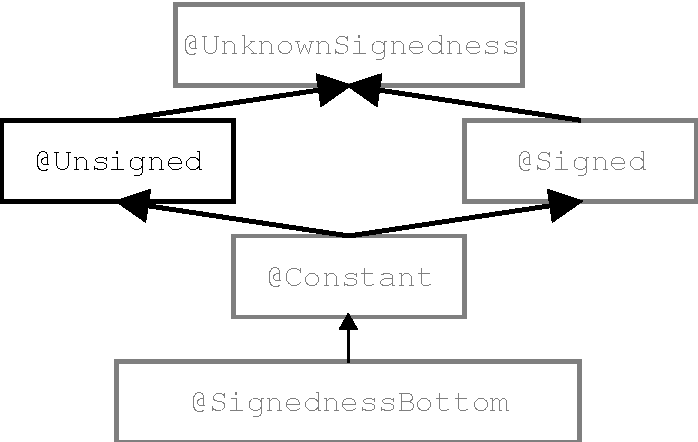
\includegraphics[width=0.4\textwidth]{signedness}
    \caption{The type qualifier hierarchy of the signedness annotations.
The default annotation is \<@Signed>.
Qualifiers in gray are used internally by the type system and need not be
written by a programmer.}
    \label{fig:type-hierarchy}
\end{figure}

We have defined a signedness type system with five type qualifiers
(Figure~\ref{fig:type-hierarchy}).  Each type qualifier is written together
with a base type; for example, \<@Unsigned int i> declares a
variable named \<i> of type \<@Unsigned int>.

\begin{itemize}\itemsep 0pt \parskip 0pt
  \item \<@Unsigned> signifies that a value is interpreted as unsigned.
  \item \<@Signed> signifies that a value is interpreted as signed.
  \item \<@Constant> is for values known at compile time, such as
    manifest literals in the source code.  The programmer might intend to
    use them as signed or as unsigned values.  Even a negative literal may
    be used as a convenience placeholder for a large positive unsigned
    integer.
  \item \<@UnknownSignedness> indicates a value for which the
    Signedness Checker has no estimate.  (This usually leads to a
    type-checking warning.)  It is also used for non-numeric
    values, which the Signedness Checker ignores.
  \item \<@SignednessBottom> indicates dead code or the \<null> value.
\end{itemize}

The programmer writes \<@Unsigned> type qualifiers within field and method
declarations in the program's source code.  Unannotated Java types within
field and method signatures are given a default qualifier (usually
\<@Signed>).  Type uses within method bodies are inferred.  More
specifically, here are the type introduction rules of our type system:

\begin{enumerate}\itemsep 0pt \parskip 0pt
  \item If the user wrote a type qualifier, use it.
  \item If an integral expression is a constant at compile time, use
    \<@Constant>.
    Integral types are \<char>, \<byte>, \<short>, \<int>, \<long>, \<Integer>, and \<Long>.
  \item Other integral expressions use \<@Signed>.
  \item Other non-integral expressions use the top type, \<@UnknownSignedness>.
\end{enumerate}

The type rules of the signedness type system issue a warning if a program
might perform a computation using operands of incorrect or mixed signedness.
These type rules are as follows:

\begin{itemize}\itemsep 0pt \parskip 0pt
  \item Unsigned values may not be used as operands for sensitive
    operators.
  \item With the exception of shifts, no operator may operate on a mix of
    Signed and Unsigned values.
  \item Logical right shifts may only be applied to unsigned values.
  \item Arithmetic right shifts may only be applied to signed values.
\end{itemize}

An insensitive operator is allowed to be used on either signed or unsigned
values, so long as all the operands are of the same type.  In general, an operator's
result type is the least upper bound of its argument types.


\section{Background and Implementation}

Our goal is to build a verification tool that guarantees that software is
free of bugs related to unsigned integers. To achieve this, our approach
must be sound:  if it issues no warnings, then the program must be free of
bugs.
This means that the tool can issue false positive alarms:  warnings about
code that will not actually go wrong at run time.  This occurs when the
Signed Checker cannot prove that the code is correct. See Figure~\ref{fig:false-alarm}
for an example of code for which the Signedness Checker may issue a false alarm.

We built our Signedness Checker implementation using the
Checker Framework~\cite{Ernst2008,DietlDEMS2011}, which enables the
construction of pluggable type systems for Java.

Our pluggable type system implementaion consists of the following parts:

\begin{itemize}\itemsep 0pt \parskip 0pt
  \item Type qualifiers are implemented declaratively as Java 8 type
    annotations~\cite{JSR308-PFD}.
  \item Type indroduction rules are defined procedurally.
  \item Type rules are enforced by a visitor which visits each node of the syntax tree.
\end{itemize}

The Signedness Checker is distributed as part of the Checker Framework
\url{http://CheckerFramework.org/}, starting with version 2.1.0.

\begin{figure}
\begin{lstlisting}

/*
 * The Signedness Checker issues a
 * warning for each of the following
 * lines because a signed int is
 * right shifted with an unsigned
 * right shift. In reality this is
 * fine because all of the introduced
 * bits are masked off.
 */

sb.data[i++] = (byte) ((c >>> 8) & 0xff);
sb.data[i++] = (byte) ((c >>> 16) & 0xff);
sb.data[i++] = (byte) ((c >>> 24) & 0xff);

\end{lstlisting}
\vspace{-10pt}
\caption{An example of code for which the Signedness Checker will issue a false
alarm, from our case study of jake2.}
\label{fig:false-alarm}
\end{figure}

\section{Results and Contributions}

To put the Signedness Checker to the test, we used it to analyze jake2, a Java
port of the popular '90s video game, Quake II. This case study is a large,
complex piece of software, with many instances of unsigned integers being used
in system code. Without applying annotations the Signedness Checker listed many
perceived errors with using a logical right shift, sometimes called an unsigned
right shift, on signed operands. Many of these were eliminated by annotating
documented unsigned integers, but a few persisted. By comparing jake2 with the
original C implementation, we have been able to identify and record semantic
differences between the two systems, particularly in the usage of right shifts.
In detail, the jake2 implementation uses logical right shifts on \<@Signed> values
in many locations where the C implementation used arithmetic right shifts. We have
identified several cases in which this difference has no actual effect, as in the
example used in Figure~\ref{fig:false-alarm}, but it
is possible that if a negative value is passed to such regions of code that the
two implementations will behave differently in a way noticible to the end-user.
Further analysis is required to determine if any of these differences have
noticeable effects. Furthermore, we have been able to identify one bug,
depicted in Figure~\ref{fig:bug}, in which
unsigned integers are passed to a utility function which prints their values during
debugging. No special handling of the unsigned values is done, so they are printed as
if signed, which can possibly lead to erroneous output for values outside signed
positive range.

\section{Conclusions}

In conclusion, we have developed a type system, the Signedness Type System, to
encapsulate all the necessary information to examine the usage of signed and unsigned
integers in Java programs. This type system is implemented with the Signedness
Checker in the Checker Framework to allow Java programs to be type checked with this
system. This allows us to statically analyze Java programs, ensuring that if they
type check under our type system, that they are free of bugs related to unsigned
integers in Java.

\begin{figure}
\begin{lstlisting}

/*
 * Both out.firstleafbrush and
 * out.numleafbrushes are Unsigned integers.
 * The method Vargs::add(int) expects a Signed
 * integer by default and therefore the
 * Signedness Checker issues a
 * warning here.
 */

if (debugloadmap) {
  Com.DPrintf("|%8x|%6i|%6i|%6i|\n",
    new Vargs()
      .add(out.contents)
      .add(out.cluster)
      .add(out.area)
      .add(out.firstleafbrush)
      .add(out.numleafbrushes));
}

\end{lstlisting}
\vspace{-10pt}
\caption{An example of code for which the Signedness Checker will issue a false
alarm, from our case study of jake2.}
\label{fig:bug}
\end{figure}

\bibliographystyle{abbrv}
\bibliography{bibstring-unabbrev,ernst,generals,invariants,types}

\end{document}

%  LocalWords:  papersize Signedness Mackie signedness javac's jake2 90s
%  LocalWords:  UnknownSignedness SignednessBottom
